\chapter{Launching a Virtual Machine at Amazon Web Services}
\label{ch:1}

\setcounter{problem}{1}

\section{Discussion}

\begin{fullwidth}

The goal of this lab is to teach you to create a Linux machine at \href{http://aws.amazon.com}{\textcolor{blue}{Amazon Web Services}}, login, copy some data to that machine, and run a simple Python program on that data.

\section{Steps}

\step Login to AWS and go to your \href{http://aws.amazon.com/console/}{\textcolor{blue}{AWS console}}.

\scalebox{.45}{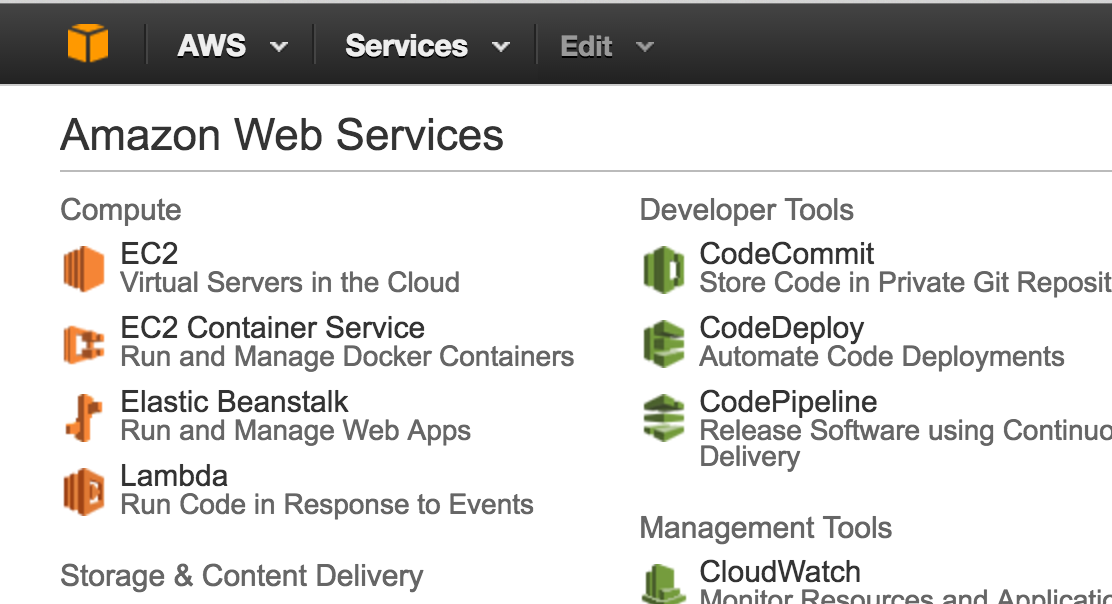
\includegraphics{figures/console_snippet.png}}

\step Click "Launch Instance", which will start the process to create a virtual machine in the cloud. An instance is just a virtual machine.

\scalebox{.75}{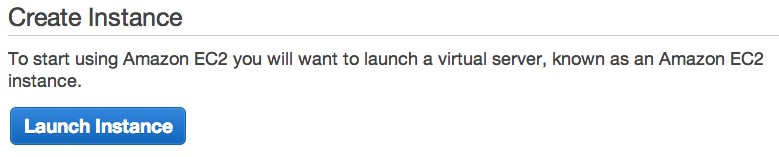
\includegraphics{figures/launch.png}}

\step Select the ``Amazon Linux AMI'' server, which should be the first one.  This is a commonly-used {\em image} that results in a Linux machine that contains lots of useful goodies as you can see from that list, such as Python and MySQL. An image is just a snapshot of the disk after someone carefully installs software properly on a Linux machine. This means we don't have to install software every time we create a new machine.

\scalebox{.75}{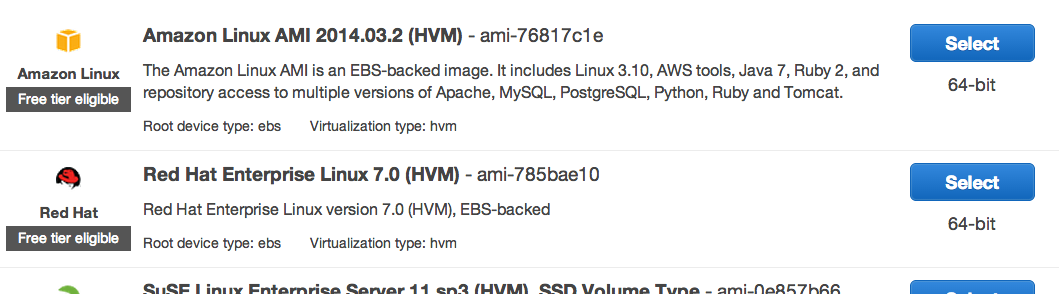
\includegraphics{figures/ami.png}}

\step Select instance type ``m1.micro,'' which should be the first machine type listed. This machine is very low powered but is sufficient for playing around. Click ``Next: configure instance details.''

\scalebox{.75}{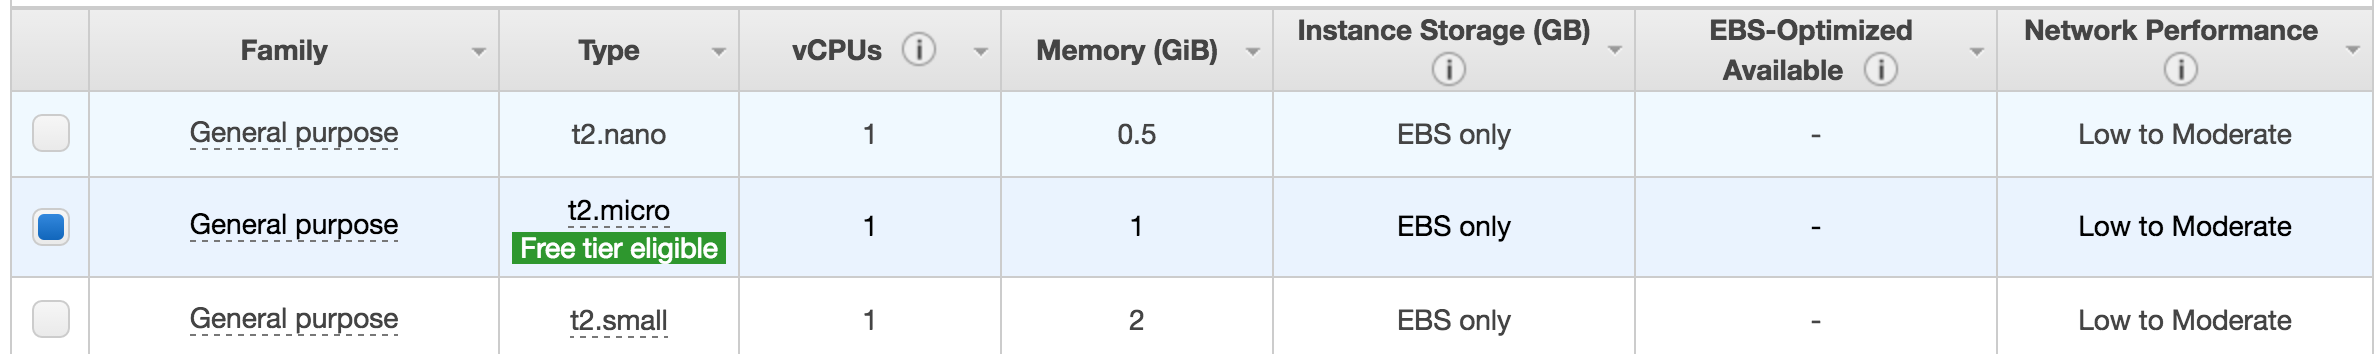
\includegraphics{figures/selectvm.png}}

\step  You can leave the configuration details as-is:

\scalebox{.75}{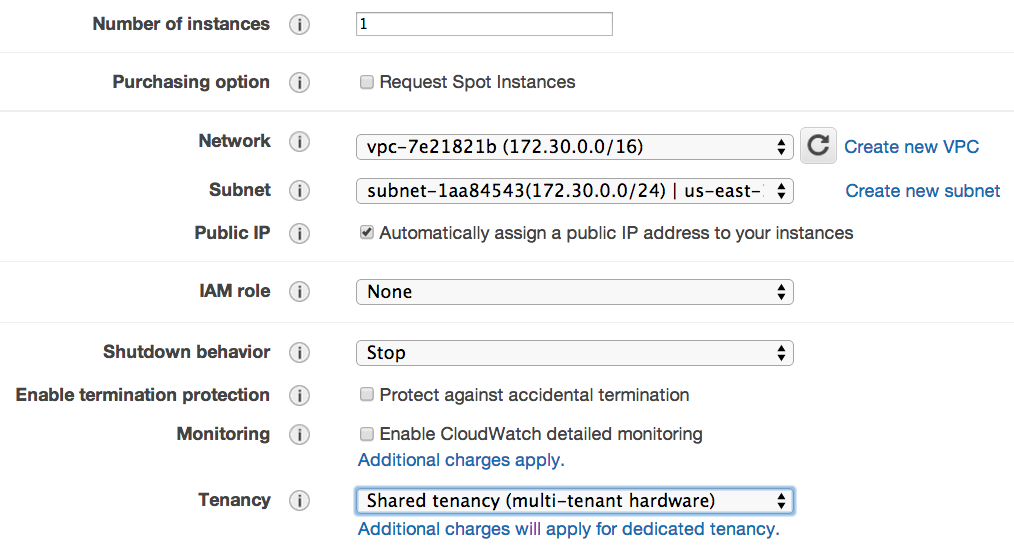
\includegraphics{figures/config.png}}

\step  Ignore the network interface set up and advanced details.  Click ``Next: Add storage.''

\step It shows that it will give us 8G of disk storage on a magnetic disk by default, which is good enough for our testing purposes.  Click ``Next: Tag instance.''

\scalebox{.75}{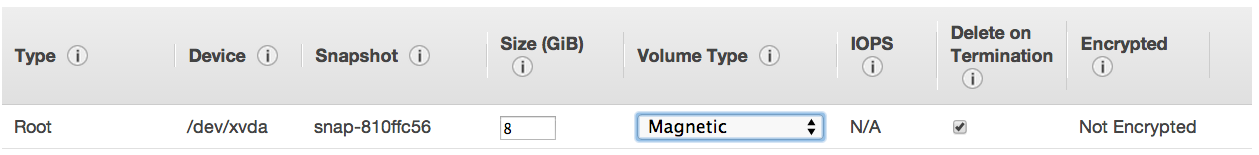
\includegraphics{figures/storage.png}}

\step For the key named "Name", change the value to something like {\em youruserid}-linux or something like that so that you can identify it later if you have multiple machines going. Click ``Next: Configure security group.'' Then click on the group whose name is ``default.'' Your list of security groups might not be the same.

\scalebox{.75}{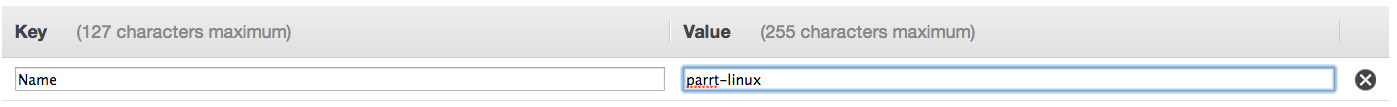
\includegraphics{figures/tag.png}}

\step You want to create a new security group, so that you learn how to deal with firewalls. We want to allow SSH access, Windows RDP, and HTTP ports.   Name it something like your userid-default. You should be able to reuse this the next time you create an instance just by selecting the name from the existing security groups pulldown. It initially shows just SSH port open so we have to add two more. 

\scalebox{.75}{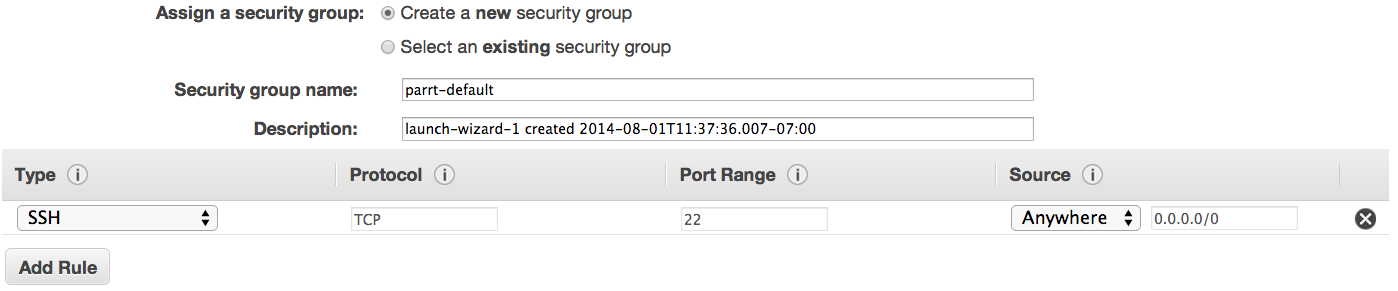
\includegraphics{figures/security-group.png}}

\step Click on the ``Add rule'' button and select RDP under the type and Anywhere under the source. That means we want anyone to be able to connect to this machine using the Windows Remote Desktop protocol and from any machine on the Internet. This is not a Windows machine but you will reuse the security group later. As we might want to start a Web server on our cloud computer, add a rule for HTTP.

\scalebox{.75}{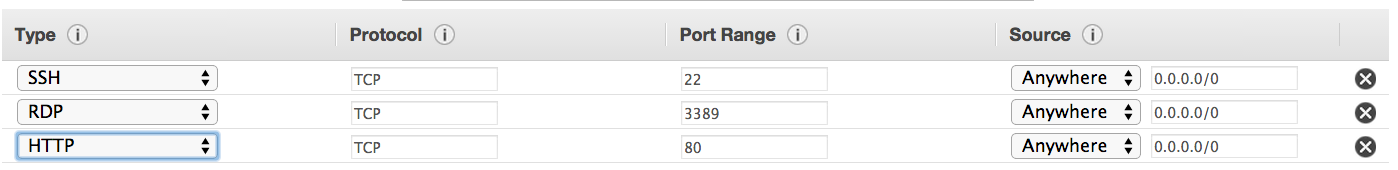
\includegraphics{figures/rdp-http.png}}

\step Click ``Review and launch,'' which will pull up a dialog box asking you to select whether you want SSD or old-school spinning magnetic disk. As we are just testing things and don't care about I/O speed, choose the magnetic disk and click ``Next.''

\scalebox{.75}{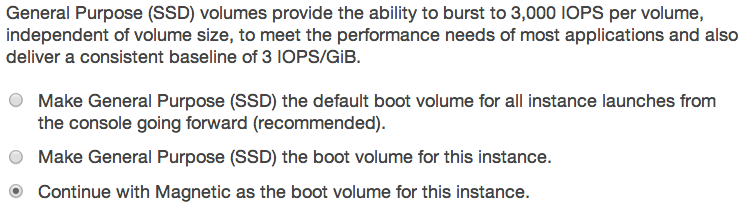
\includegraphics{figures/magnetic.png}}

\step Click ``Launch,'' which will bring a dialog box up to select a key pair. A key pair is what allows you to securely access the server and prevent unauthorized access. The first time, you will need to create a new key pair. Name it as your user ID then click on ``Download key pair.'' It will download a {\em userid}.pem file, which are your security credentials for getting into the machine. Save that file in a safe spot. If you lose it you will not be able to get into the machine that you create.

\scalebox{.75}{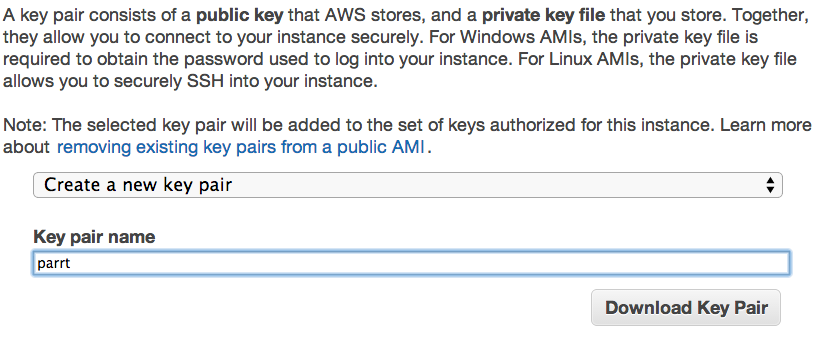
\includegraphics{figures/keypair.png}}

\step Click on the ``I acknowledge that I have ...'' checkbox then ``Launch instances.'' You should see something like:

\scalebox{.75}{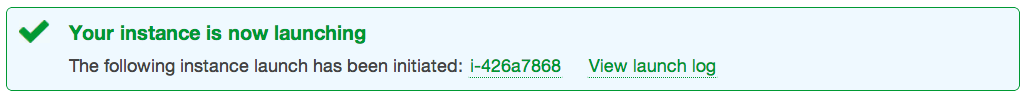
\includegraphics{figures/launched.png}}

\step Click on the ``i-...'' link to go to the EC2 console showing your instance.

\scalebox{.75}{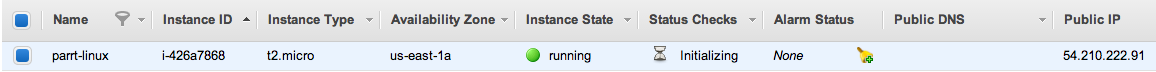
\includegraphics{figures/ec2-instance.png}}

\step Click on your instance and you should see a description box at the bottom. Look for the ``Public IP'' address, which is 54.210.222.91 in this case:

\scalebox{.75}{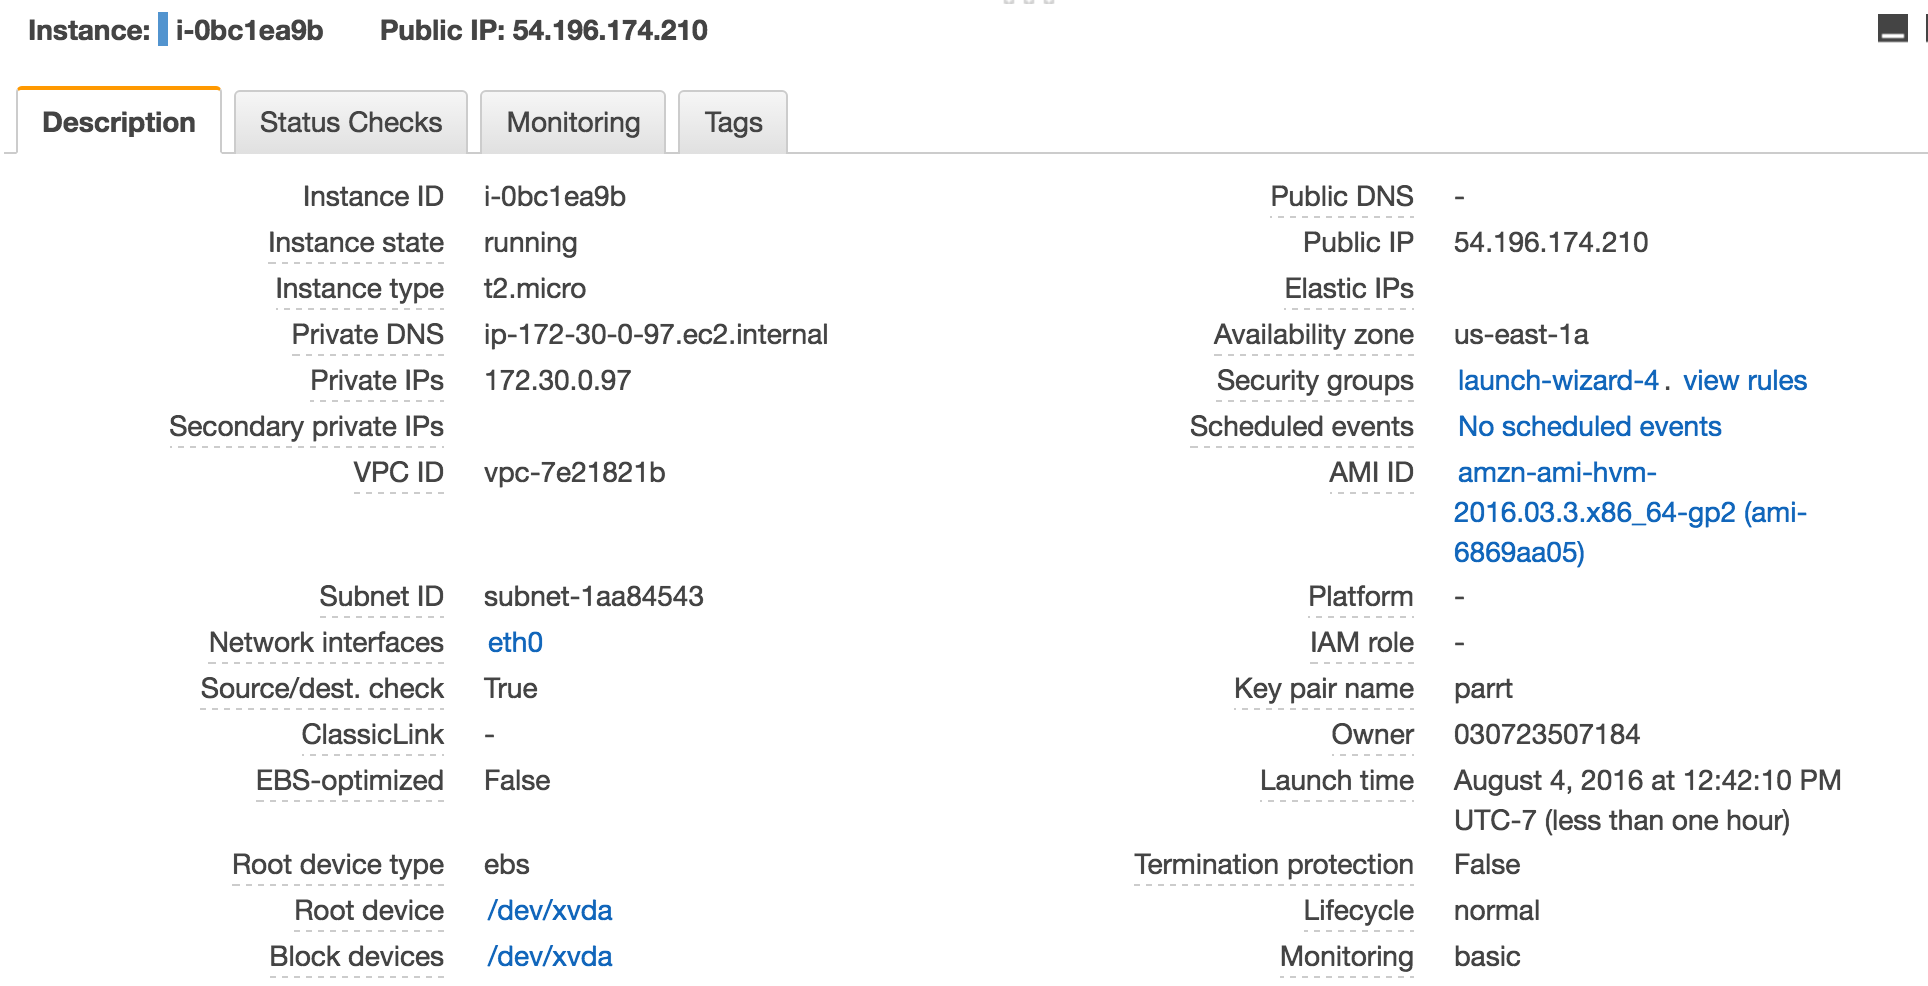
\includegraphics{figures/publicIP.png}}

\step Click on the ``Connect'' button at the top of the page and it will bring up a dialog box that tells you how to connect to the server.  You want to connect with ``A standalone SSH client'' link (Java is now a security risk in the browser so we can't use that choice.)  Inside you will see the {\tt ssh} command necessary to connect to your machine. If you have Windows, there is a link to show you how to use an SSH client called PuTTY. 

\scalebox{.75}{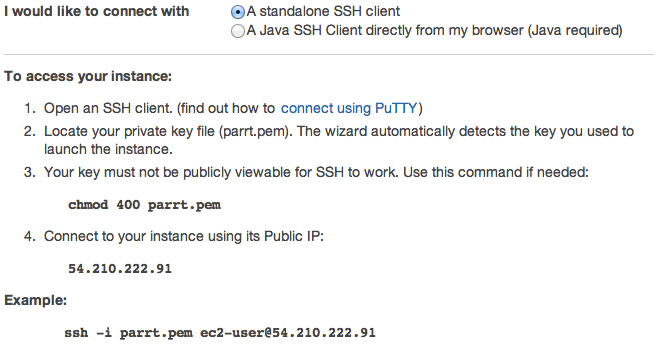
\includegraphics{figures/connect.png}}

For mac and linux users, we will use the direct {\tt ssh} command from the command line. It will be something like:

{\small
\begin{alltt}
ssh -i ~/Dropbox/licenses/parrt.pem ec2-user@54.210.222.91
\end{alltt}
}

\noindent Naturally, you will have to provide the full pathname to your user.pem file.

\step  Before we can connect, we have to make sure that the security file is not visible to everyone on the computer (other users). Otherwise ssh will not let us connect because the security file is not secure:

{\small
\begin{alltt}@@@@@@@@@@@@@@@@@@@@@@@@@@@@@@@@@@@@@@@@@@@@@@@@@@@@@@@@@@@
@         WARNING: UNPROTECTED PRIVATE KEY FILE!          @
@@@@@@@@@@@@@@@@@@@@@@@@@@@@@@@@@@@@@@@@@@@@@@@@@@@@@@@@@@@
Permissions 0644 for '/Users/parrt/Dropbox/licenses/parrt.pem' are too open.
It is required that your private key files are NOT accessible by others.
This private key will be ignored.
bad permissions: ignore key: /Users/parrt/Dropbox/licenses/parrt.pem
Permission denied (publickey).
\end{alltt}
}

\noindent Whoa!  Do this:

{\small
\begin{alltt}
$ cd ~/Dropbox/licenses
$ ls -l parrt.pem
-rw-r--r--@ 1 parrt  parrt  1696 Aug  4 15:15 /Users/parrt/Dropbox/licences/parrt.pem
\end{alltt}
}

\noindent To fix the permissions, we can use whatever ``show information about file'' GUI your operating system has or, from the command line, do this:

{\small
\begin{alltt}
cd ~/Dropbox/licenses
chmod 600 parrt.pem
\end{alltt}
}

\noindent which changes the permissions like this:

{\small
\begin{alltt}
$ ls -l parrt.pem
-rw-------@ 1 parrt  501  1696 Aug  1 12:12 /Users/parrt/Dropbox/licenses/parrt.pem
\end{alltt}
}

\noindent Don't worry if you don't understand exactly what's going on there. It's basically saying that the file is only read-write for me, the current user, with no permissions to anybody else.

\step  Try to connect again and it will now warn you that you have never connected to that machine before. Again, this is a security measure. You can simply say ``yes'' here.

{\small
\begin{alltt}
ssh -i ~/Dropbox/licenses/parrt.pem ec2-user@54.210.222.91
The authenticity of host '54.210.222.91 (54.210.222.91)' can't be established.
RSA key fingerprint is 49:1d:f6:ff:1a:19:5d:00:bb:cd:43:c1:84:ee:8e:a6.
Are you sure you want to continue connecting (yes/no)? yes
Warning: Permanently added '54.210.222.91' (RSA) to the list of known hosts.
\end{alltt}
}

\noindent Once you connect, you should see the following output from the terminal:

{\small
\begin{alltt}
       __|  __|_  )
       _|  (     /   Amazon Linux AMI
      ___|\___|___|

https://aws.amazon.com/amazon-linux-ami/2014.03-release-notes/
8 package(s) needed for security, out of 19 available
Run "sudo yum update" to apply all updates.
[ec2-user@ip-172-30-0-201 ~]$ 
\end{alltt}
}

\noindent The \$ is your prompt just like you have on your local machine using the terminal / shell.

\step To get data up to the server, you can cut-and-paste if the file is small. For example,  cut-and-paste the following data into a file called {\tt coffee} in your home directory. First copy this data from the PDF:

{\small
\begin{alltt}
3 parrt
2 jcoker
8 tombu
\end{alltt}
}

\noindent then type these commands and paste the data in the sequence:

{\small
\begin{alltt}
$ cd ~ # get to my home directory
$ cat > coffee
3 parrt
2 jcoker
8 tombu
^D
$ cat coffee # print it back out
3 parrt
2 jcoker
8 tombu
$ 
\end{alltt}
}

\noindent The {\tt \^{}D} means control-D, which means end of file.  {\tt cat} is reading from standard input and writing to the file. The way it knows we are done is when we signal in the file with control-D.

\step For larger files, we need to use the secure copy {\tt scp} command that has the same argument structure as secure shell {\tt ssh}. Get another shell up on your laptop. From the directory where you have the {\tt coffee} file on your laptop, use the following similar command:

{\small
\begin{alltt}
$ scp -i ~/Dropbox/licenses/parrt.pem access.log ec2-user@54.210.222.91:~ec2-user
access.log                                    100% 1363KB   1.3MB/s   00:00
$ 
\end{alltt}
}

\noindent {\em Do not forget the {\tt :\textasciitilde ec2-user} on the end of that line.} The {\tt access.log} file is at github under labs/data.  From the shell that is connected to the remote server, ask for the directory listing and you will see the new file:

{\small
\begin{alltt}
$ ls
access.log  coffee
$ 
\end{alltt}
}

\step Play around with your instance and then {\em TERMINATE YOUR INSTANCE WHEN YOU ARE DONE}, otherwise you will continue to get charged for the use of that machine. If you right-click on the instance and say "Stop", it will stop the machine and you still get charged but you can restart it without having to go through this whole procedure. If you say "Terminate", it will toss the machine out and you will have to go through this procedure again.

\section{Deliverables}

None. Please follow along in class.

\end{fullwidth}
